% <- percent signs are used to comment
\documentclass[titlepage,12pt]{article}

%amsmath is a packaged use for typesetting math
%amsfonts is required for special fonts, e.g. blackboard bold (for denoting real numbers, etc.)
\usepackage{amsmath,amsfonts}

\usepackage{fullpage,url,amssymb,epsfig,color,xspace}

\title{Assignment 4}
\date{June 17, 2015}
\author{Jerry Jiang\\ TianQi Shi}

%Note: Many of the packages above have other uses beyond those used in this document

%this marks the beginning of the document. Everything before this is called the Preamble.
\begin{document}
\maketitle

\section*{A}

\subsection*{RL Circuit}

The original equation for the RL Circuit is:

$$E(t) = Ri(t) + Li'(t)$$
To get the state space for the simulation, we start by defining a differential equation:

$$i(t) = x(t)$$
If we differentiate both sides, we get

$$i'(t) = x'(t)$$
Which can be expanded to
$$\frac{E(t) - Ri(t)}{L} = x'(t)$$
So,
$$\frac{E(t) - Rx(t)}{L} = x'(t)$$
We substitute this into the state space vector. Below is the MATLAB code used in this simulation.

\begin{verbatim}
% RLCircuit.m

function dx = RLDamper(t, x, w, r, l)
% Generates the RL Circuit equation sin(wt) = ri(t) + li'(t)
% t is the time
% x is the current
% w is the frequency in rad/sec
% r is the resistance
% l is the inductance

xd1 = (sin(w*t) - r*x(1)) / l % first order derivative

dx = [xd1];

end

% solver.m

clc; clear all; close all;

% Solve the RLCircuit function under different conditions

% Parameters
r = 10 % resistance
l = 0.1; % inductance
w= 4*r/l; % frequency
t_max = 5; % simulation time = 5s

x_0 = 0; % initial current

X_0 = [x_0];

[t,y] = ode45(@RLCircuit, [0, t_max], X_0, [], w, r, l);

plot(t, y(:,1));
xlabel('Time (sec.)');
ylabel('Current (charge/sec)');
title('RLCircuit Systems');

\end{verbatim}

\section*{B}

\subsection*{RL Circuit}
We initially start off with the following graph, using initial conditions
$R = 10$, $L = 0.1$, and $w = 2\pi$.
\begin{center}
  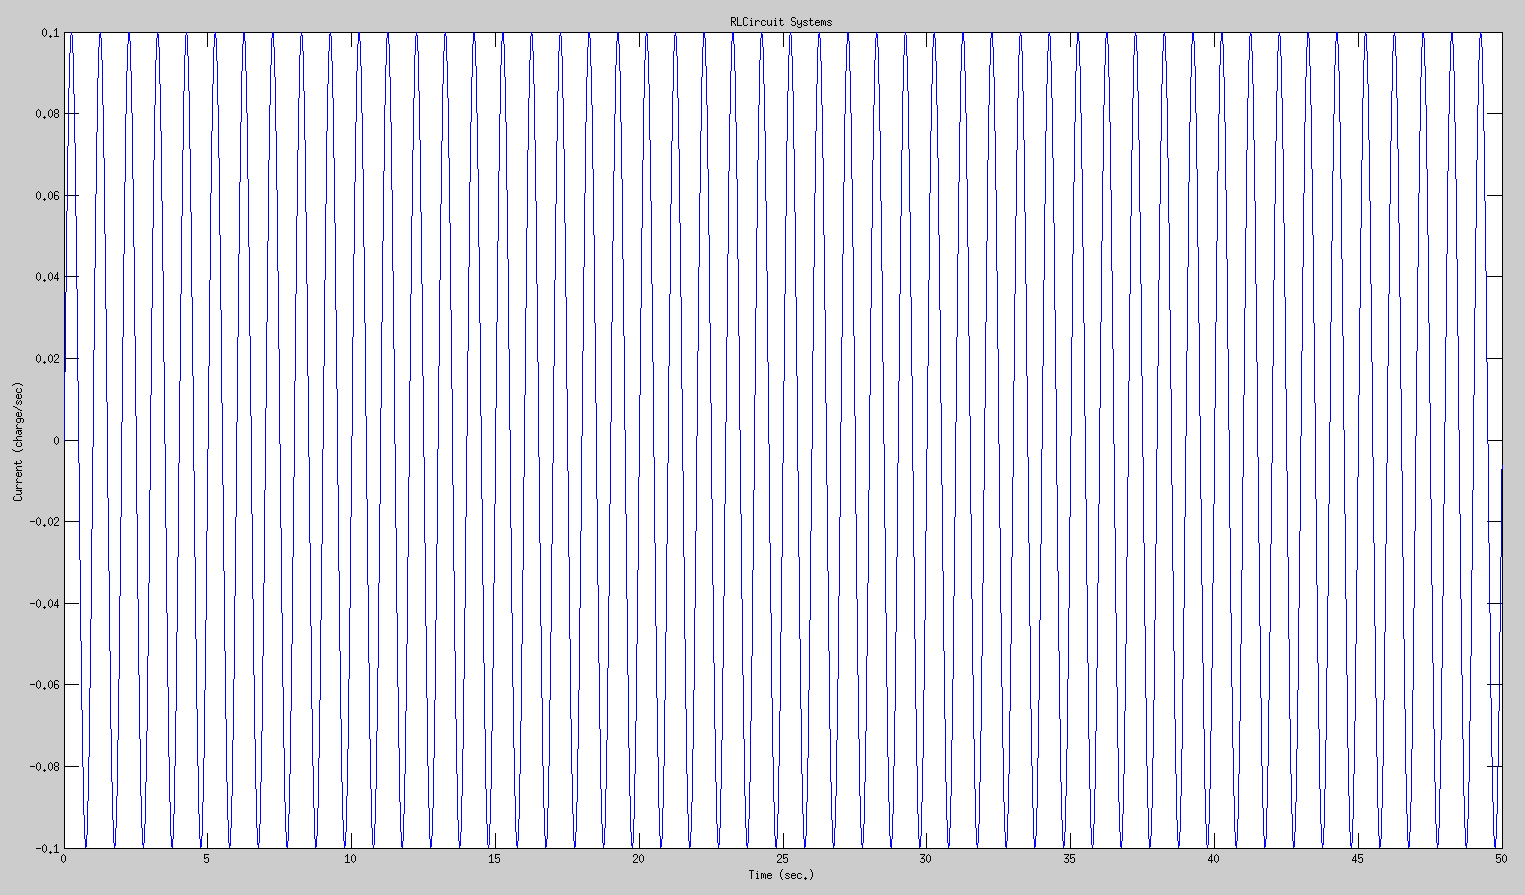
\includegraphics[scale=0.25]{r10l01w2pi.png}
\end{center}

\noindent Next we decrease the resistance such that $R = 0.001$.

\begin{center}
  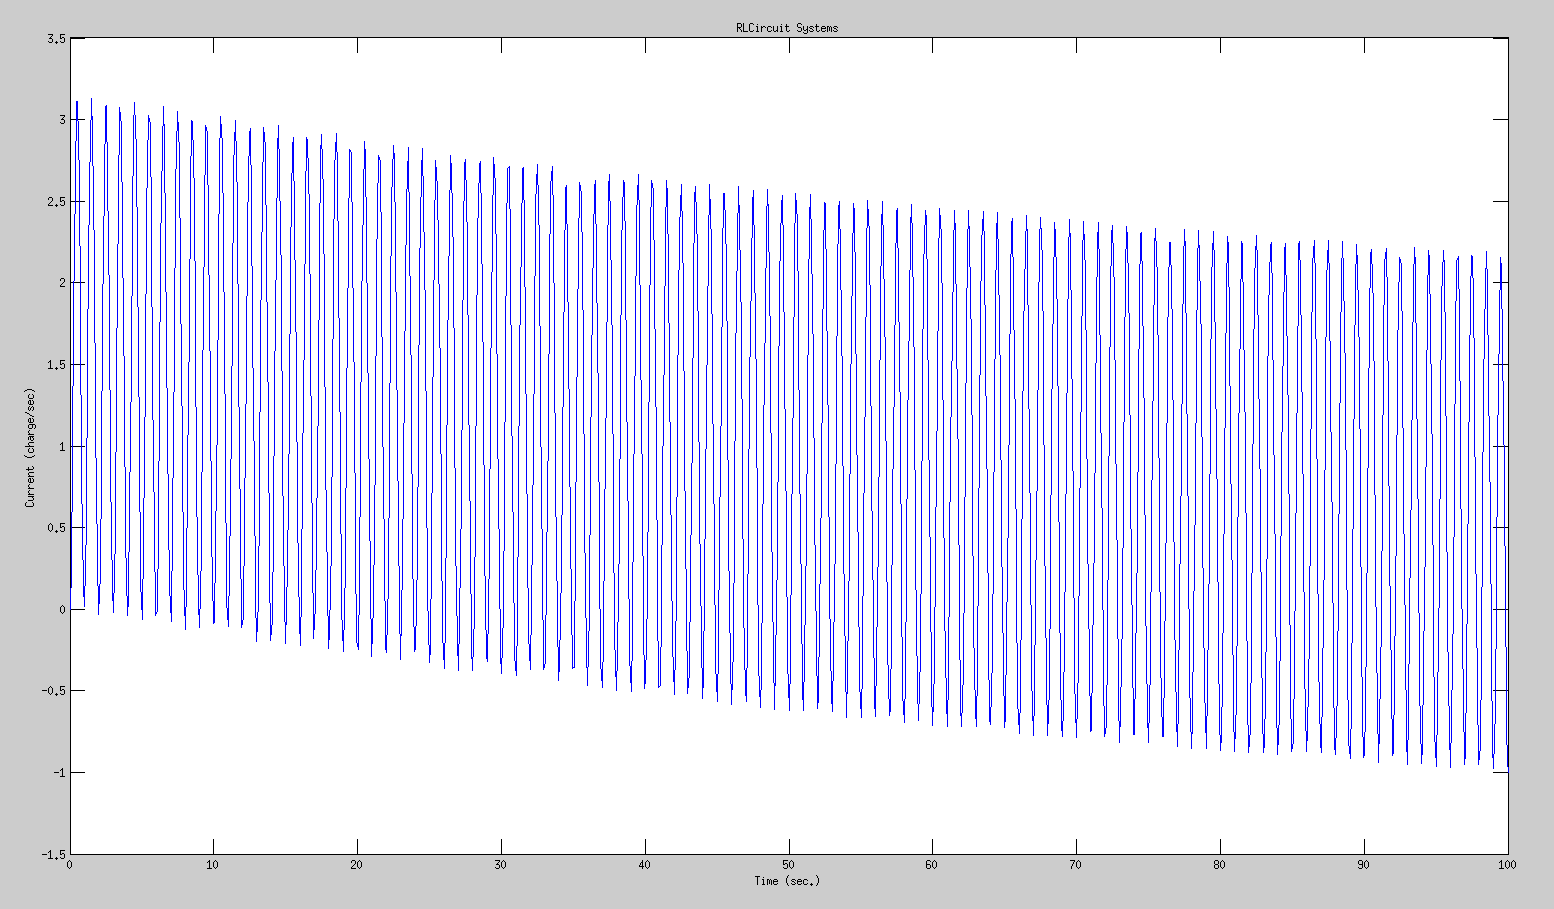
\includegraphics[scale=0.25]{r0001l01w2pi.png}
\end{center}

\noindent From this graph, we can see that the amplitude of the current is increased from below 0.1 to above 1.5. This makes sense, because the lower the resistance of the circuit, the higher the current can be for a given voltage. Next we increase the resistance such that $R = 1000$.

\begin{center}
  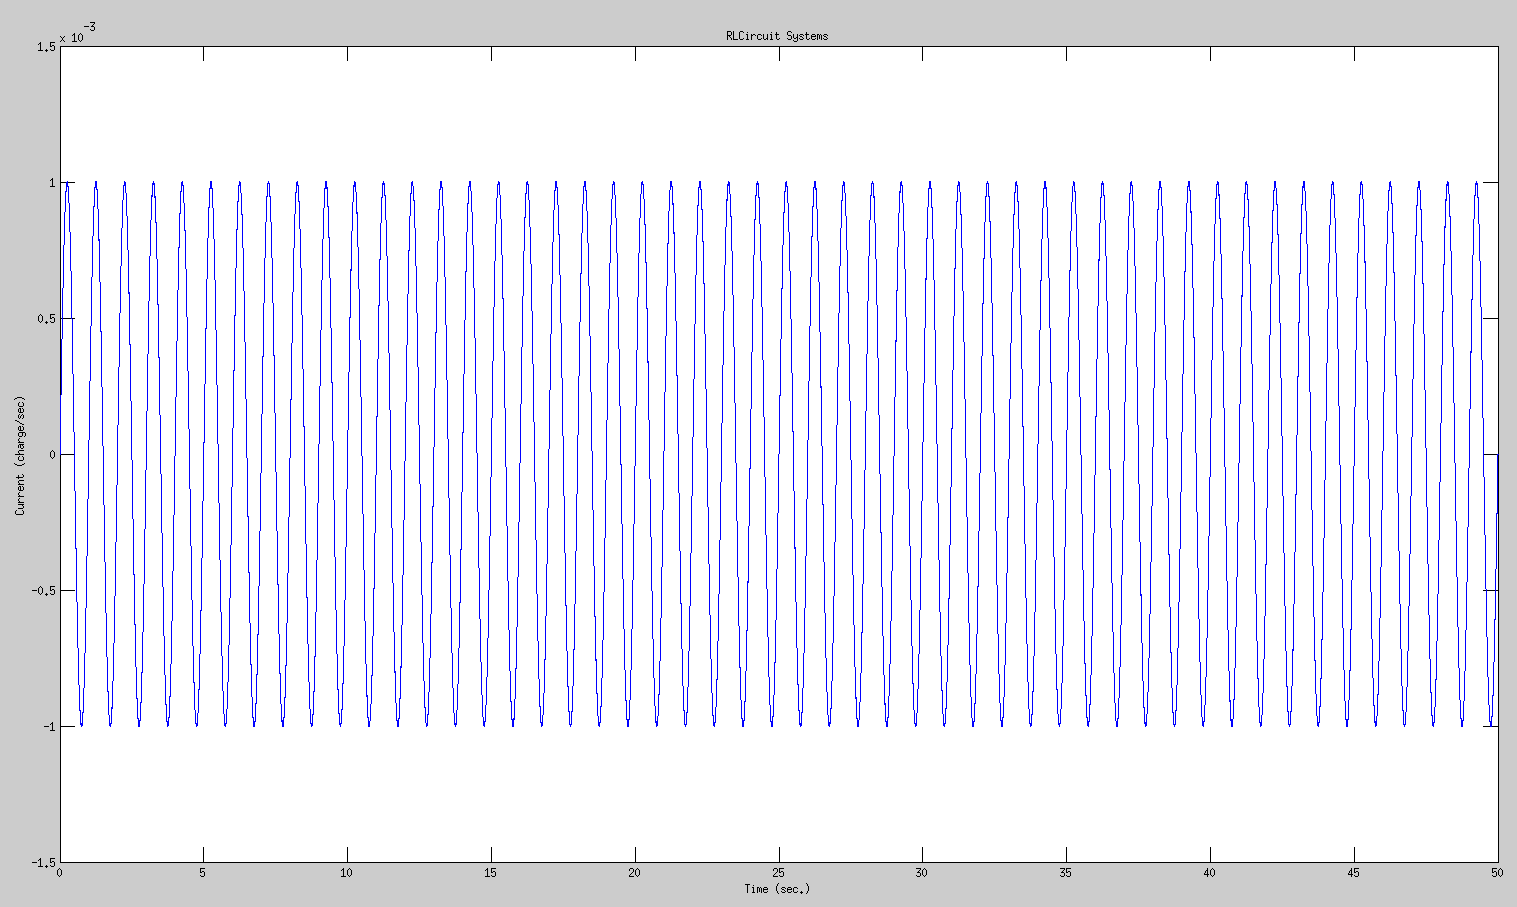
\includegraphics[scale=0.25]{r1000l01w2pi.png}
\end{center}

\noindent We get a really small amplitude, as the resistance is very high. This also makes sense, because Ohm's law dictates that as resistance increases, current should decrease. Next, we set the resistance back to $R = 10$ and vary the frequency, starting at the baseline of $w = R/L$.

\begin{center}
  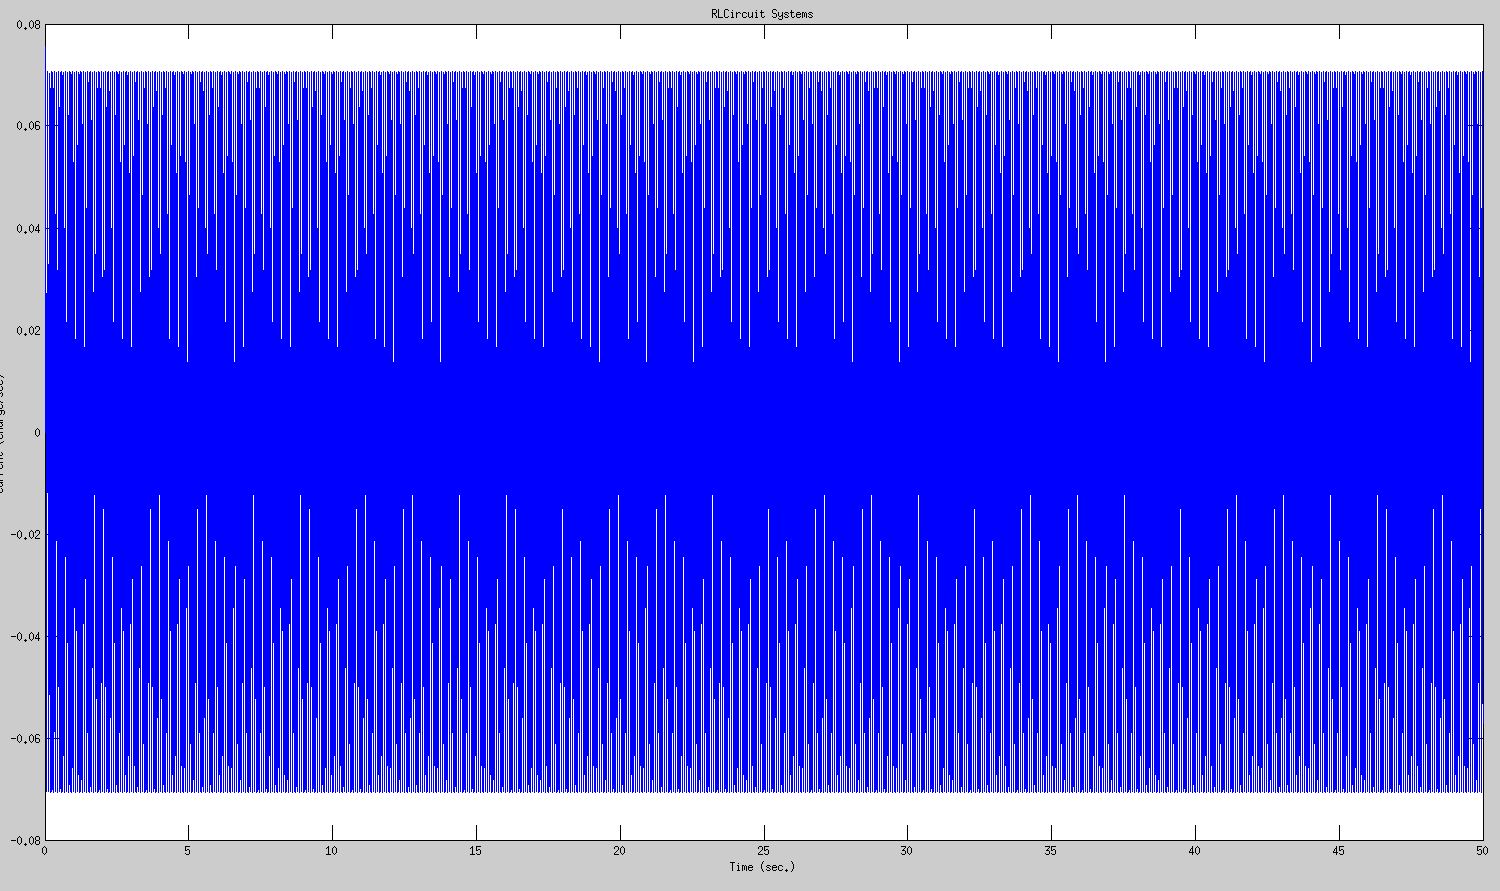
\includegraphics[scale=0.25]{r10l01wrl.png}
\end{center}

\noindent In this graph, you can see that beating occurs, as there are multiple layers of sinusoidal waves. Next, we lower the frequency down to $w = 0.25R/L$.

\begin{center}
  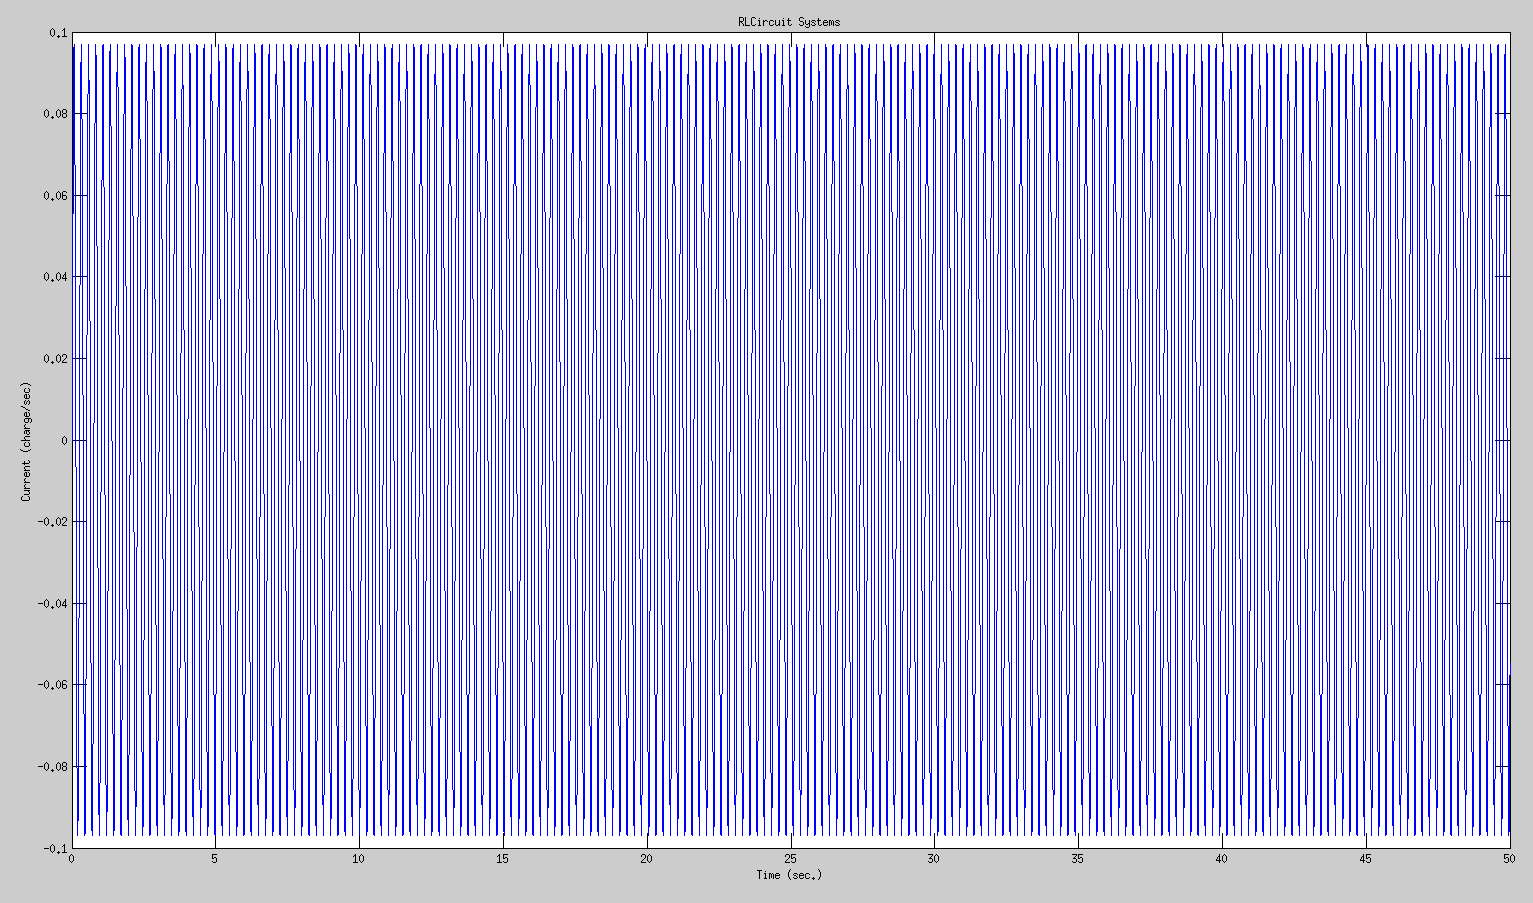
\includegraphics[scale=0.25]{r10l01w025rl.png}
\end{center}

\noindent Beating still occurs, but the important fact is that the amplitude of the current has increased. Next, we increase the frequency to $w = 4R/L$.

\begin{center}
  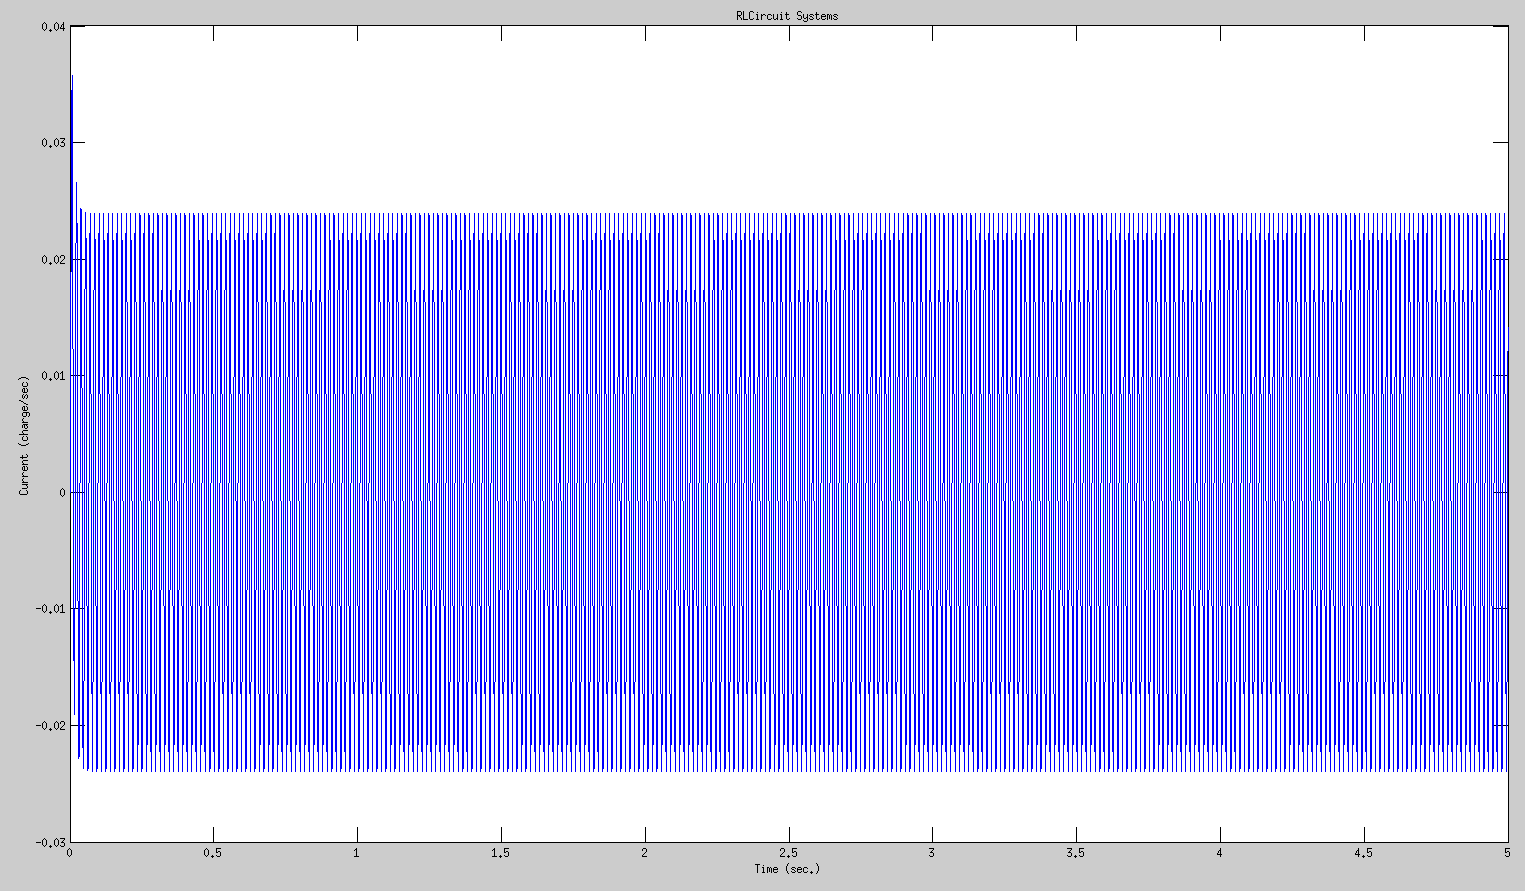
\includegraphics[scale=0.25]{r10l01w4rl.png}
\end{center}

\noindent Beating, again, still occurs, but we can see that increasing the frequency has decreased the amplitude of the wave. Overall, it seems that the amplitude of the circuit scales inversely proportional to the frequency of the forcing function.

\section*{C}

\subsection*{RL Circuit}
\noindent This circuit could be used in a subwoofer, because it seems to be able to amplify lower frequencies while de-amplifying higher frequencies. A subwoofer is designed for lower frequency sounds, so having the circuit able to trim out the unwanted higher frequency noises would make it very suitable for use in a subwoofer.

\pagebreak
\section{RCL Circuit}

First we derive the differential equation for the system.
$$E(t) = L \frac{d^2q}{dt^2} + R\frac{dq}{dt} + \frac{q}{C}$$
To get the state space for the simulation, we start by defining two linear differential equations.
$$y_1(t) = x(t)$$
$$y_2(t) = x'(t)$$
If we differentiate both sides,
$$y_1'(t) = x'(t) = y_2(t)$$
$$y_2'(t) = \frac{E(T)}{L}-\frac{R}{L} x' - \frac{1}{CL}x$$
We substitute these into the state space vector. Below is the MATLAB code used in the simulation:
\begin{verbatim}
% MSDamper.m
function dx = MSDamper(t,x,l,c,r)

xd1 = x(2); %%first order derivative
%% note that c is actually 1/capacitance so we must use inverse
xd2 = sin(t)/l-(r/l)*x(2) - (c/l)*x(1);  %%second order derivative

dx = [xd1; xd2];
end
\end{verbatim}

\begin{center}
        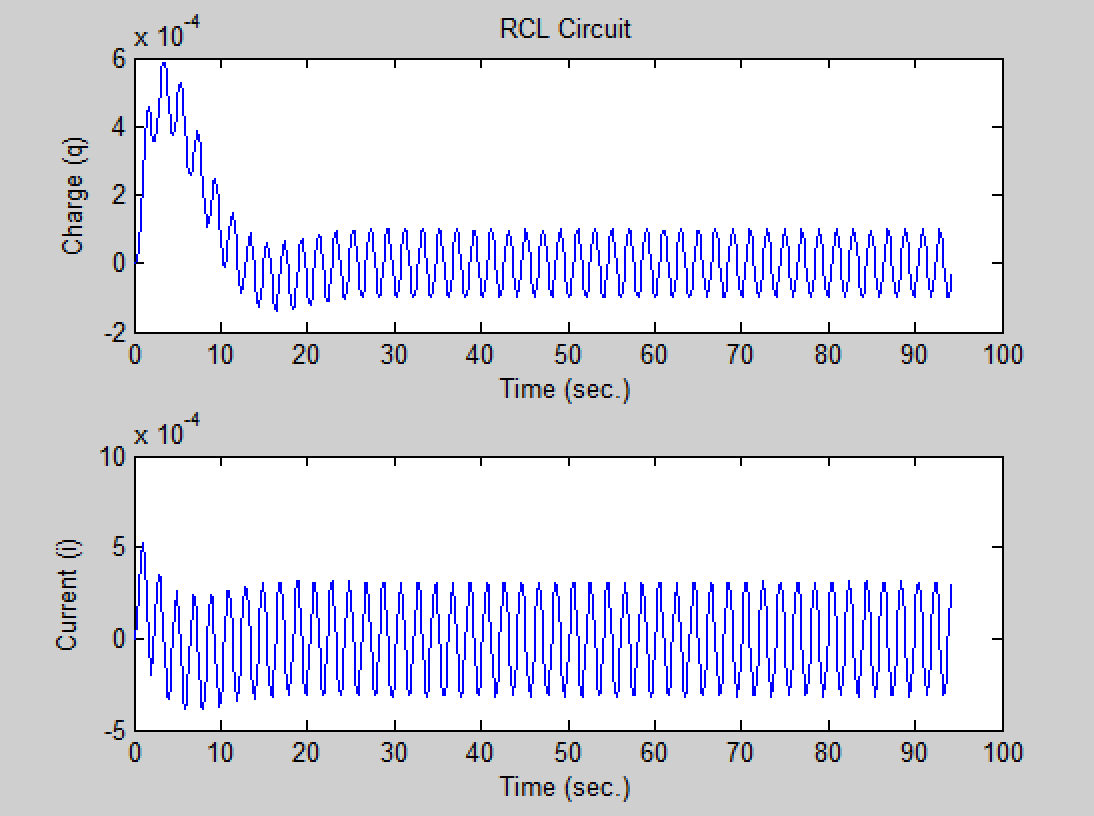
\includegraphics[scale=0.6]{base.png}
\end{center}

\noindent The above graph is a good representation of the base case. A transient is present towards the beginning of the graph but due to damping, end behaviour is an oscillation around 0. This signal is due to our sinuoidal input signal.

\begin{center}
        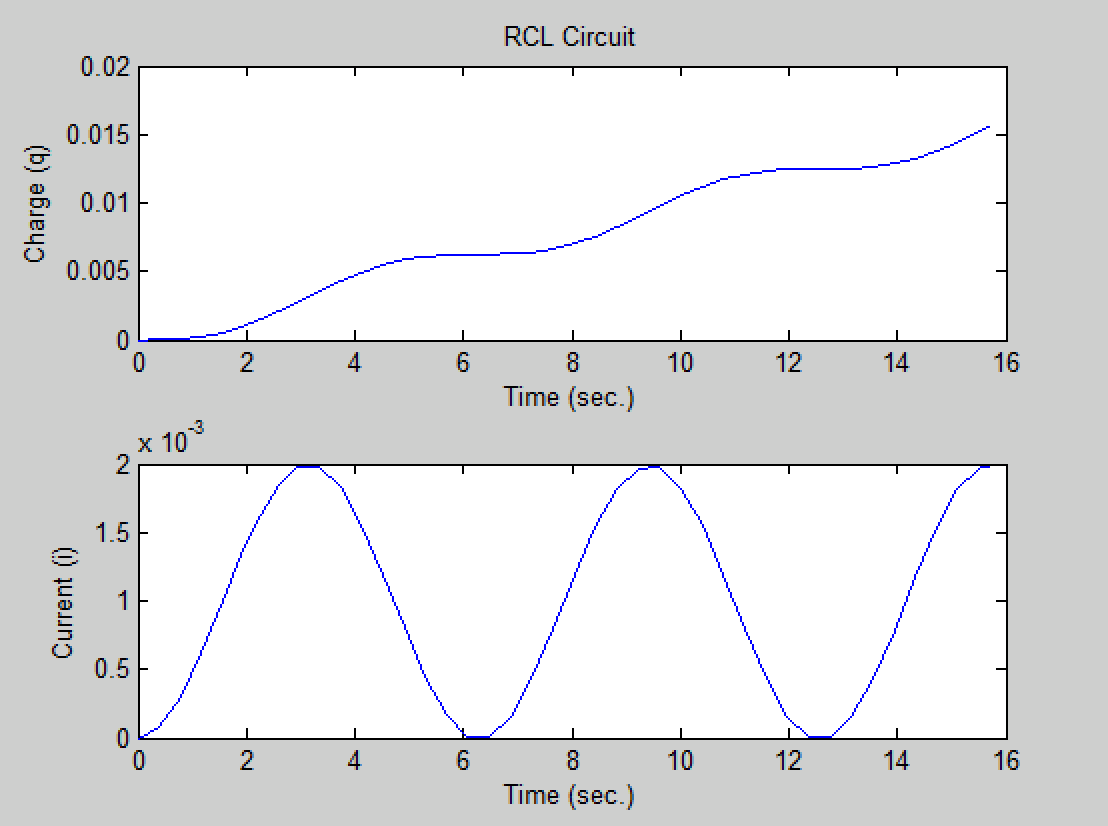
\includegraphics[scale=0.6]{rcl-lowr.png}
\end{center}

\noindent In our first variation, we have a very low resistance value compared to inductance and capacitance. We can see that the graph is not damped and has infinity for end behaviour.

\begin{center}
        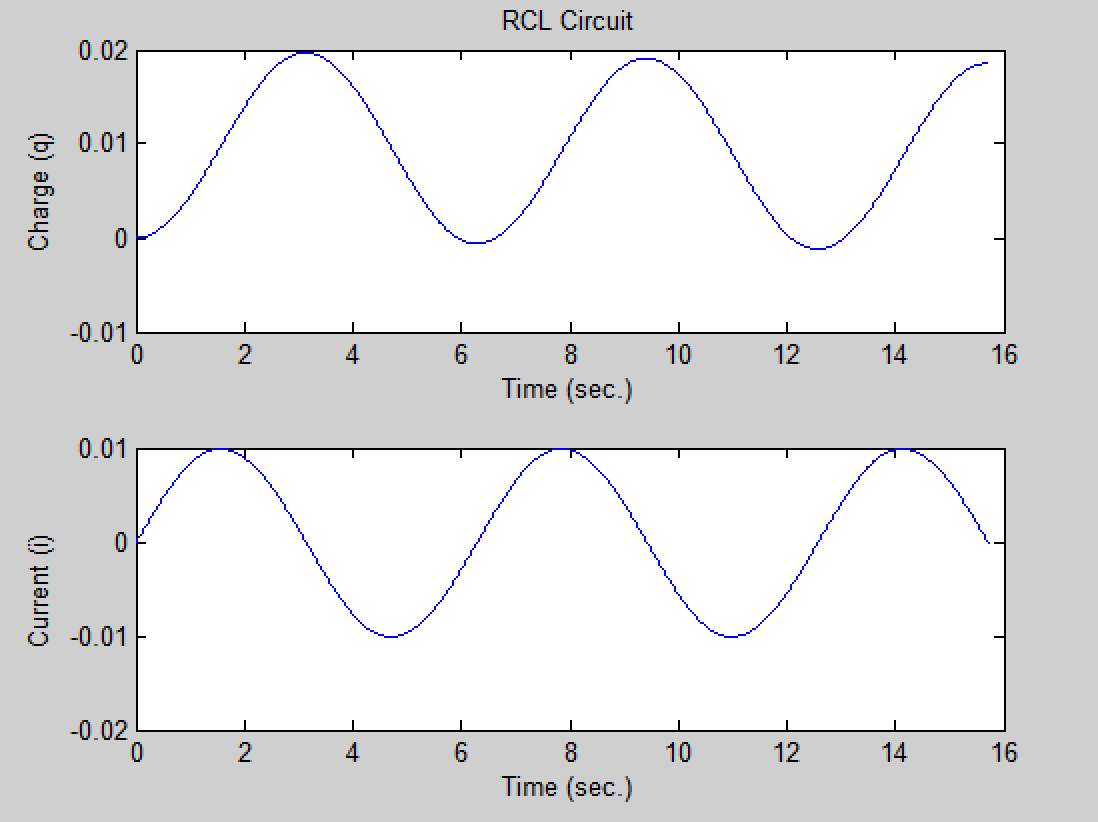
\includegraphics[scale=0.6]{rcl-highr.png}
\end{center}

\noindent Conversely, when resistance is very high relative to inductance and capacitance, the system does not experience damping and stays around input level amplitudes.

\begin{center}
        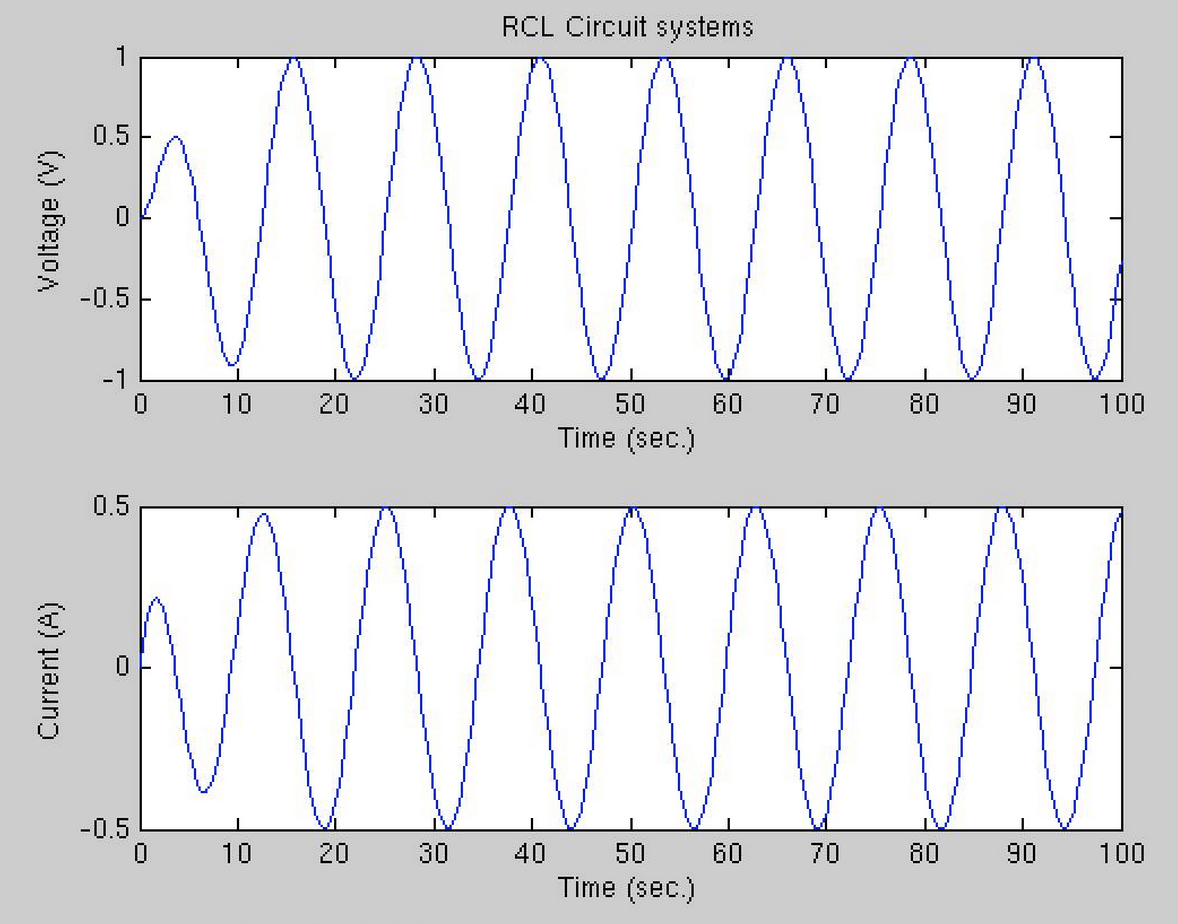
\includegraphics[scale=0.6]{resonance.png}
\end{center}

\noindent We observe that when the frequency is exactly $\sqrt{\frac{1}{CL}}$, there is a resonance phenomenon which causes the signal to grow. This can be used to pick up signals transmitted at certain frequencies as something with the same frequency will have a very high signal while all other frequencies will be damped. When transmitters on cell phones send signals, the signal is sent at a specific frequency so the receiver will get various frequencies signals. Applying this resonance concept allows it to select whatever is useful to itself.

\end{document}
